\documentclass[12pt]{article}

\usepackage{graphicx}
\usepackage{url}
\usepackage{color}
\usepackage{fancyhdr}
\usepackage[T1]{fontenc}
\usepackage[polish]{babel}
\usepackage[utf8]{inputenc}
\usepackage{lmodern}
\usepackage{caption}
\usepackage{listings}
\selectlanguage{polish}
\title{My first document}
\author{Kamil Warpechowski}

\setlength\parindent{24pt}


\fancypagestyle{firststyle}
{
   \fancyhf{}
   \fancyfoot[C]{
		Warszawa, \today
   }
}

\usepackage{color}
\definecolor{bluekeywords}{rgb}{0.13,0.13,1}
\definecolor{greencomments}{rgb}{0,0.5,0}
\definecolor{redstrings}{rgb}{0.9,0,0}


\lstset{language=[Sharp]C,
  showspaces=false,
  showtabs=false,
  breaklines=true,
  showstringspaces=false,
  breakatwhitespace=true,
  escapeinside={(*@}{@*)},
  commentstyle=\color{greencomments},
  keywordstyle=\color{bluekeywords},
  stringstyle=\color{redstrings},
  basicstyle=\ttfamily
}

\begin{document}


\thispagestyle{firststyle}
\begin{center}

\includegraphics[width=1\textwidth]{images/logo.jpg}
\textbf{Wydzial Informatyki} \\
\vspace{3em}
\textbf{Katedra Sieci Komputerowych} \\
Sieci Urządzeń Moblinych \\
\vspace{3em}
\textbf{Kamil Warpechowski} \\
Nr albumu 10709
\end{center}


\vspace{3em}
{\addtolength{\leftskip}{70mm}

\noindent
Praca inżynierska
\\Promotor:
\\dr inż. Michał Tomaszewski

}

\vspace{3em}

\textbf {
	tutaj będzie zajebisty tytuł
}



  \newpage
  
  
  \tableofcontents
  \newpage
  

\section{Cel pracy}
Celem niniejszej pracy jest stworzenie platformy do budowania gier oraz interaktywnych animacji prezentowanej za pomocą rozszerzonej rzeczywistości sterowaniej za pomocą zdalnego kontrolera.

Przykłady zastosowanie zestawu aplikacji:

\begin{itemize}
\item Prezentacje przestrzeni architektonicznych
\item Rozrywka
\item Reklama miejscach użyteczności publicznych (np. centra handlowe)
\end{itemize}

\section{Rozszerzona rzeczywistość}
Natural Machines, Meta2
\begin{center}
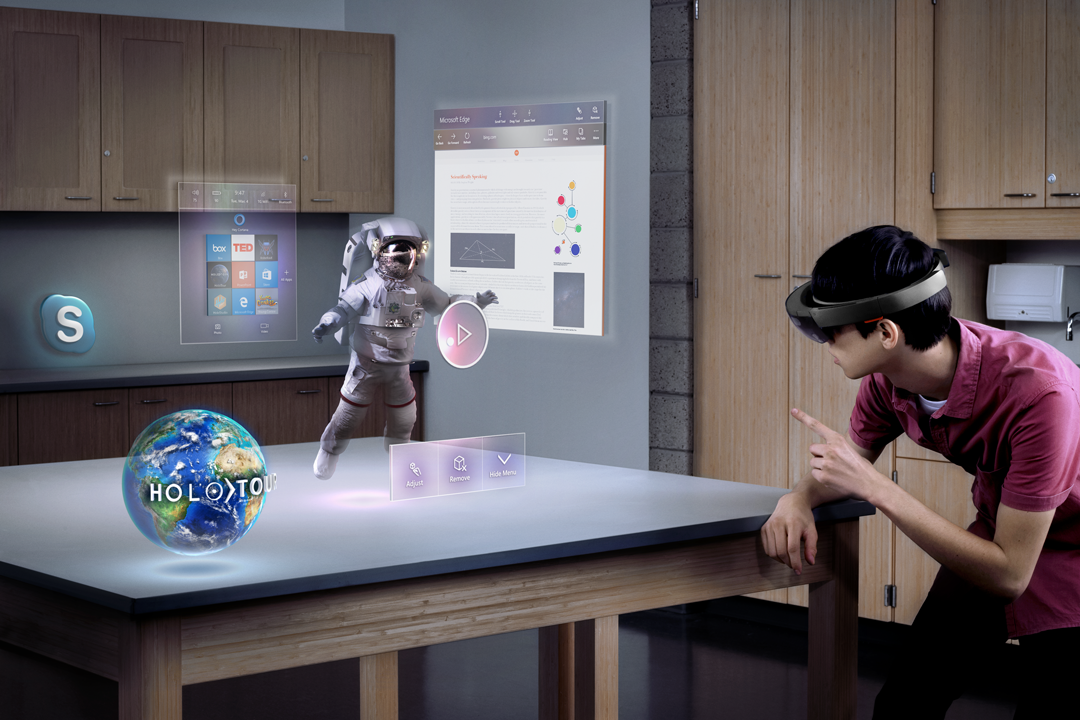
\includegraphics[width=0.8\textwidth]{images/hololens.png}
\captionof{figure}{
Wizualizacja Microsoft HoloLens
}
\small {źródło: https://www.microsoft.com/microsoft-hololens/en-us/why-hololens }
\end{center}

\section{Wykorzystane technologie}

\subsection{Unity}
Unity jest obecnie najpopularniejszą platformą do tworzenia gier na wiele platform. 
\subsubsection{Dlaczego Unity}
Najnowsza wersja posiada natywne wsparcie do rozszerzonej oraz wirtualnej rzeczywistości. Narzędzie te posiada prosty, ergonomiczny interfejs co ułatwia pracę.\\
Bardzo pomocnym dodatkiem do narzędzia jest ,,Assets Store''. Jest to wirtualny sklep z komonentami do tworzenia gry. W projekcie zastosowałem tekstury i obiekty 3d pochodzące z tego źródła.
\subsubsection{Alternatywne rozwiązania}
 \begin{tabular}{|c|c|c|}
 \hline
 \ & Unity & Unreal Engine \\ 
  \hline
 Wsparcie języków programowania & C\#, JavaScript, Boo & c++ \\  
  \hline
 Obsługa wielu ekranów & Tak & Nie \\
 \hline  
  &  &  \\
  \hline   
  &  &  \\
  \hline   
  &  &  \\
  \hline   
\end{tabular}
\captionof{table}{Porównanie silników gier}

\subsubsection{Wybór języka programowania}
Środowisko Unity wspiera obsługę skryptów (animacje oraz logika biznesowa) w kilku językach programowania: C\#, UnityScript (zmodyfikowana wersja JavaScript)  oraz w przeszłości Boo. Podjąłem decyzję, by w projekcie użyć język C\#, gdyż ów język jest najbardziej stabilny, posiada najbardziej rozbudowaną dokumentację oraz jest to najbardziej popularny język w specjalistycznej literaturze. Dodatkowym udogodnieniem  jest to, iż  język posiada wiele wbudowanych klas (np. do obsługi połączęń TCP) oraz niezliczoną ilość zewnętrznych bibliotek.
\subsubsection{Unity IDE}
Środowisko Unity jest multiplatformowe. Aplikacje można używać na dowolnym sytemie operacyjnym. Jednakże edycja skryptów odbywa się za pomocą zewnętrznego narzędzia. W systemie Mac OS X jest to MonoDevelop, natomiast w systemie Windows jest to VisualStudio w wersji Community. Opisywana aplikacja początkowo była tworzona na systemie Mac OS X, jednakże kołopoty ze środowiskiem MonoDevelop spowodwały decyzje o przeniesieniu środowiska na system Windows. Subiektywnie mogę stwierdzić, że stabilność oraz komfort pracy jest dużo lepszy w systemie Windows.
Dodatkową alternatywą dla MonoDevelop może okazać się Visual Studio Code. Jest to prosty multiplatformowy edytor posiadający obsługę języka C\# .

\subsubsection{Licencja i koszty}
Unity jest zamkniętym, licencjonowanym oprogramowaniem. Darmowa wersja (Personal Editon) pozwala na nielimitowane użycie, jednakże jest to okrojona edycja. Szersze informacje o ograniczeniach wersji Personal zawarte są w kolejnych rozdziałach. Licencja pozwala na komercyjne użycie przy limicie zarobków na poziomie stu tysięcy dolarów.
Komercyjna wersja (Professional Edition) jest płatna w modelu subskrybcyjnym (75 dolarów za miesiąc)\footnote{https://store.unity3d.com/subscribe}.
Na potrzeby opisywanego projektu zasotosowano Unity w wersji Personal Edition.

\subsection{Android}
Naturalnym wyborem technologii przy tworzeniu aplikacji na urządzenie sterujące byłoby Unity, gdyż te środowisko pozwala na kompilacje kodu na urządzenia mobilne(systemy iOs, Android, Windows Phone, Tizen). Jednakże Unity w wersji Personal Edition nie pozwala na uruchomienie warstwy sieciowej na urządzeniach mobilnych.
Na potrzeby implementacji przykładowego urządzenia sterującego wybrano platformę Android, gdyż ma ona największy udzła w rynku. Proces tworzania aplikacji na tą platformę przebiega w języku Java.

\subsubsection{Android Studio}

\subsection{Komunikacja sieciowa}
Największym wyzwaniem było stworzenie dwukierunkowego protokołu komunikacyjnego pomiędzy serwerem (aplikacja napisana w środowisku Unity) oraz dowolnym kontrolerem lub w przyszłości innym urządzeniem wysłającym dane do aplikacji. Podstawowym założeniem było to iż, kontrolerem gry może być standardowy telefon komórkowy. Dodatkowo w przyszłości planowana jest rozbudowa o zdalne sterowanie za pomocą przeglądarki internetowej. Pierwotnie ozważane było użycie Bluetooth, jednak ograniczyłoby to zdalne sterowanie. Podjęto decyzję projektową o użyciu połączenia sieciowego. Rozważano następujące protokoły:

\subsubsection{UNET}
Unity wspiera natywną obsługę multiplayer - UNET, jednakże jest to zamknięty protokół. Komunikacja możliwa jest tylko pomiędzy aplikacjami stworzonymi w tym środowisku.

\subsubsection{HTTP (SOAP, REST)}
Komunikacja za pomocą HTTP (protokoły komunikacyjne takie jak np. SOAP, REST) są bardzo często spotykane. Jest to standard aplikacji internetowych. HTTP nadaje się do przesyłu dużych wolumenów danych, jednak niezbyt dobrze sprawdza się przy małych, lecz częstych połązeniach pomiędzy klientem, a serwerem. Duży narzut czasowy może spowodować transormacja danych do oraz z formatu JSON lub XML. Jednakże dużą zaletą wspomnianych protokołów jest prostota implementacji w większości języków programowania, gdyż są już gotowe komponenty.
\subsubsection{TCP}
{\color{red}Opisać, że TCP jest ogólnie lepsze - socket, ale to jest nadal połączeniowy, więc lepiej by było udp}
\subsubsection{UDP}
{\color{red}opisać, ze to najlepsze rozwiazanie - bezpolazeniowe}

\newpage
\section{Aplikacja główna}


{\color{red}tutaj będą makiety}

\subsection{Świat gry}
\subsection{Aktorzy}

\begin{center}

 \begin{tabular}{|c|c|}
 \hline  
  &   \\
  \hline   
  &   \\
  \hline   
\end{tabular}
\captionof{table}{Właściwości aktora}


\end{center}

\begin{lstlisting}
public void SendInfo() {
	Network.SendMessage("hasax_"+this.hasAx);
	Network.SendMessage("hassh_"+this.hasSh);
	Network.SendMessage("hasdrabina_"+this.drabina);
	Network.SendMessage("isMove_"+this.isMove);
}
\end{lstlisting}


\subsection{Kamery}
Platforma Unity wspiera do 8 wirtualnych kamer \footnote{http://docs.unity3d.com/Manual/MultiDisplay.html}.
Każda z tych kamer może być prezentowana na oddzielnym fizycznym ekranie.


\subsection{Logika biznesowa}
\subsection{Serwer komunikacyjny}
\section{Aplikacja mobilna - kontroler}

\section{Środowisko uruchomieniowe}
Powyżej opisana aplikacja została uruchomiona testowo w labolatorium na Polsko-Japońskiej Akademii Technik Komputerowych.

\subsection{Serwer}
Serwer został uruchomiony na komputerze przenośnym(laptop) posiadającym kartę graficzną umożliwiajacą podłączenie dwóch zewnętrznych ekranów - projektorów. Pierwszy z nich został połączony za pomocą złącza cyfrowego HDMI, natomiast drugi łączem DVI.
\subsection{Aplikacja mobilna - kontroler}

\section{Dalszy rozwój}

 
\newpage
\thispagestyle{empty}
 
  
\listoffigures
 
\listoftables
\begin{thebibliography}{99}
\bibitem{pa} Building Microservices,  Sam Newman , Wydanie 4, 2016
\end{thebibliography}

\end{document}
